\documentclass[border=4pt]{standalone}
\usepackage{tikz}
\usetikzlibrary{arrows,arrows.spaced,positioning}
\begin{document}
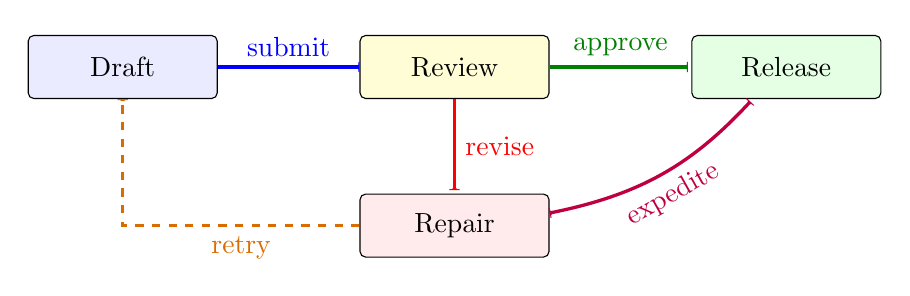
\begin{tikzpicture}[
  node distance=12mm and 18mm,
  stage/.style={draw,rounded corners=2pt,minimum width=24mm,minimum height=8mm,align=center},
  route/.style={line width=1.2pt}
]
  \node[stage,fill=blue!8] (draft) {Draft};
  \node[stage,fill=yellow!16,right=of draft] (review) {Review};
  \node[stage,fill=green!10,right=of review] (release) {Release};
  \node[stage,fill=red!8,below=of review] (repair) {Repair};

  \draw[route,blue,-{serif cm}] (draft) -- node[above]{submit} (review);
  \draw[route,green!50!black,-{spaced serif cm}] (review) -- node[above]{approve} (release);
  \draw[route,red,-{spaced serif cm}] (review) -- node[right]{revise} (repair);
  \draw[route,dashed,orange!85!black,-{serif cm}]
    (repair.west) -| node[pos=.25,below]{retry} (draft.south);
  \draw[route,purple,{serif cm}-{spaced serif cm}]
    (repair) to[bend right=18] node[below,sloped]{expedite} (release);
\end{tikzpicture}
\end{document}
